\documentclass[titlepage]{article}

 % Dans le préambule
%\usepackage[style=author]{biblatex} % package de bibliographie, on cite l’auteur
%\addbibresource{Bib2Validation.bib} % notre fichier bib exporté

%%%%% Tous les packages
\usepackage[left=2cm,right=2cm,top=2cm,bottom=2cm]{geometry}
\usepackage[utf8]{inputenc}% accents in
\usepackage[french]{babel}% typo française
\usepackage[T1]{fontenc}% accents out
\usepackage{lmodern}
\usepackage{titlepic}
\usepackage[noae]{Sweave} % "noae" permet à Sweave de reconnaitre les guillemets
\usepackage[%
    all,
    defaultlines=3 % nombre minimum de lignes
]{nowidow} % éviter les lignes orphelines

% package maths
\usepackage{amsmath}
\usepackage{amsfonts}
\usepackage{amssymb}
\usepackage{ dsfont } %proba
\usepackage{ stmaryrd }
% tables et figures
\usepackage{longtable}
\usepackage{subfigure}
\usepackage{lscape}
\usepackage{multirow} % permet de fusionner les colonnes
\usepackage{graphicx} % admet les figures
\usepackage{array} % types particuliers de tableaux
\usepackage{tabularx} % autres tableaux, notamment pour gérer les doubles traits de séparation (voir hhline)
\usepackage{listings} % pas forcément utile ici, mais permet de faire des box avec du code
\usepackage[hang,font = normalsize, labelfont=bf,textfont=bf]{caption} % mise en forme du caption
% hyperlinks
\usepackage{hyperref}
\hypersetup{ %moduler les couleurs des liens
    colorlinks=true,
    linkcolor=black,
    % filecolor=magenta,      
    urlcolor= blue,
    citecolor = black
}
\usepackage{indentfirst} % Pour indenter les premiers paragraphes de section
%kableExtra
\usepackage{booktabs}
\usepackage{longtable}
\usepackage{array}
\usepackage{multirow}
\usepackage{wrapfig}
\usepackage{float}
\usepackage{colortbl}
\usepackage{pdflscape}
\usepackage{tabu}
\usepackage{threeparttable}
\usepackage{threeparttablex}
\usepackage[normalem]{ulem}
\usepackage{makecell}
\usepackage{xcolor}
\usepackage{hyperref} %pour les liens url
%\usepackage[absolute,overlay]{textpos}

\usepackage{enumitem} % pour gérer l'espacement vertical dans les listes


%Pour la biblio
\usepackage[french]{babel}

\usepackage[backend=biber, style=apa, maxcitenames=1, natbib]{biblatex}

\usepackage{csquotes}

\setlength\bibitemsep{0.5\baselineskip}
\addbibresource{Aussant_Forcadell_Sessego_biblio.bib}



% Pour ne pas que la mention "Chapter" apparaisse à chaque chapitre mais juste le titre du chapitre
\usepackage{titlesec}
\titleformat{\chapter}{\normalfont\LARGE}{\thechapter.}{30pt}{\LARGE\bf}
\titleformat{\section}
  {\normalfont\fontsize{15}{15}\bfseries}{\thesection}{1em}{}
\titlespacing*{\chapter}{0pt}{1.1\baselineskip}{\baselineskip}



% Ne pas sauter de page entre deux chapitres

\usepackage{tcolorbox}



% titres
\title{\centering 

\vspace{1 cm}

{\begin{minipage}\linewidth
        \centering
     \textbf{Un effet inattendu du confinement : une chute de la surmortalité violente chez les jeunes ?} \\[1 cm] 
        \vspace{0.5cm}
        \large Abel Aussant, Eliot Forcadell et Ariane Sessego\\
         M2 Quantifier en Sciences Sociales\\
        \vspace{0.5cm}
         \textit{Identification causale} - Cours d'Olivier Godechot \\
         Année académique 2021-2022\\
    \end{minipage}}
  }
\date{}
%box

\begin{document}
\Sconcordance{concordance:Aussant_Forcadell_Sessego.tex:Aussant_Forcadell_Sessego.Rnw:%
1 116 1 1 19 31 1 1 16 3 1 1 10 1 7 55 1}

\Sconcordance{concordance:Aussant_Forcadell_Sessego.tex:Aussant_Forcadell_Sessego.Rnw:%
1 116 1 1 19 31 1 1 16 3 1 1 10 1 7 55 1}

\maketitle

\cleardoublepage%

En 2020, les épisodes de confinements ont bouleversé la vie des Français. Ces restrictions de sortie en dehors du domicile avaient pour but de protéger les plus vulnérables du virus de la Covid-19, particulièrement les personnes âgées, qui ont tout de même connue une forte surmortalité \parencite{breton_levolution_2022,pison_covid-19_2022,papon_bilan_2021}. Mais on peut se demander s'ils n'ont pas aussi eu des effets inattendus : le confinement a-t-il entrainé une diminution de la mortalité chez les jeunes ? \\

En effet, le risque de décès entre 15 et 30 ans est souvent plus élevé que l'on ne pourrait s'y attendre face à l'augmentation exponentielle de la mortalité habituellement constatée entre 10 et 60 ans \parencite{remund_surmortalite_2021}. On désigne donc comme "surmortalité" cet excès par rapport au risque de décès attendu, qui a longtemps été considéré comme uniquement masculin, car il était avant tout observé parmi les jeunes hommes et lié à des causes violentes de décès (accidents, homicides...) que l'on attribuait à des turbulences hormonales et de développement biologiques propre au sexe masculin \parencite{heligman_age_1980,goldstein_secular_2011}. Ces théories développementalistes ont été largement remises en question, du fait des variations de cette tendance dans le temps et l'espace ; on considère aujourd'hui cette surmortalité comme avant tout liée à des contextes socio-historiques particuliers \parencite{remund_surmortalite_2021}. En France aujourd'hui, bien qu'elle touche aussi les jeunes femmes, cette surmortalité est bien plus importante parmi les hommes, avec en moyenne trois fois plus de décès masculins que féminin à ces âges \parencite{breton_levolution_2019, pison_france_2021}, même si cette écart tend à se réduire. Elle est avant tout caractérisée par une part importante de morts violentes (accidents, homicides ou suicides) qui sont l'origine de 80\% des décès à ces âges, tout particulièrement les accidents de la circulation \parencite{remund_surmortalite_2021}. \\

Le confinement a théoriquement réduit l'exposition à ces risques, à l'exception du suicide. A-t-il entraîné une diminution de la mortalité au sein de cette population ? Le deuxième confinement, moins restrictif que le premier, a-t-il eu un impact plus faible sur cette mortalité ? \\

La méthode de différence de différence (DD) nous offre la possibilité de comparer la mortalité des jeunes adultes avant et pendant les périodes de confinement en prenant en compte la saisonnalité de la mortalité et une éventuelle variation de mortalité propre à 2020. En effet, il s'agit ici d'évaluer l'effet d'un "traitement" - le confinement généralisé de la population - sur un groupe traité - les jeunes adultes. En l'absence d'expérience aléatoire, nous ne disposons pas de groupe contrôle; et comme toute la population étant supposée confinée, il semble difficile d'en construire un. Mais nous pouvons procéder autrement pour construire un contrefactuel, notamment en considérant les périodes précédentes. Cela suppose cependant que l’évolution de la mortalité dans la population cible (les jeunes adultes) est comparable entre période. Or, on sait que la mortalité connait des tendances saisonnières importantes : la mortalité des jeunes adultes, en particulier, connait deux pics annuels, un plus faible en hiver (en février particulièrement), qui suit la tendance générale de la population, l'autre plus important en été (en juillet), qui est lié à une augmentation estivale de mortalité par accidents (Breton, 2019). Ces tendances nous empêche de comparer simplement la période pré-confinement à la période de confinement. La DD nous permet, en supposant que l'évolution de la mortalité est comparable d'une année sur l'autre, de comparer la mortalité en 2020 (groupe traité) et pendant les années précédentes (groupe contrôle), avant les confinements (période précédent le traitement) et durant chaque confinement (période de traitement), afin de mettre en avant un eventuel effet causal du confinement sur la mortalité des jeunes adultes. \\

Après une présentation des données et quelques analyses descriptives, nous présenterons en détail les modèles choisis, pour ensuite commenter les résultats. \\


\begin{tcolorbox}
 \begin{center}
 \textbf{\large Une analyse reproductible, un script disponible en ligne}
 \vspace{0.5mm}
 \end{center}
Ce travail a été réalisé par l'intermédiaire de RSweave, permettant d'intégrer des analyses statistiques effectuées avec R dans un fichier LaTeX. Le fichier permettant de produire ce rapport ainsi que la base de donnée et son fichier de recodage sont  disponible en ligne sur Github à l'adresse suivante \url{https://github.com/eliotforcadell/confinement_surmortalite}. L'analyse est donc entièrement reproductible, dans un souci de d'ouverture de la recherche et de ses résultats.
 \end{tcolorbox}

\section*{Données et méthode}



\subsubsection*{Les décès d'individus de 18 à 29 ans par date, en France métropolitaine, de 2014 à 2020}

Pour répondre à ces questions, nous utilisons les données d'état civil mises à disposition par l'INSEE, répertoriant les personnes décédées par date de décès, année de naissance, sexe, et lieu de décès pour les années 2014 à 2020 (INSEE 2014 à 2020, voir Sources, \ref{source}). Nous disposons du jour, du mois et de l'année de décès pour 2018 à 2020, mais uniquement du mois et de l'année de décès pour 2014 à 2017. \\

Nous considérons ici les décès d'individus âgés de 18 à 29 ans (age révolu au moment du décès), afin de prendre en compte la population de jeunes adultes en âge de conduire, les accidents de la circulation étant parmi les premières causes de décès chez les jeunes (INSERM, 2020) et le risque qui aurait le plus diminué durant le confinement. Nous avons de plus fait le choix de ne considérer que les décès survenus en France métropolitaine, d'une part car la littérature concernant les Outre-mer est plus rare et il est fort probable que la mortalité ne suive pas les mêmes tendance, étant donné la différence des saisons et des périodes de congé, et d'autre part car l'application du confinement, particulièrement pour le deuxième, y a été différente. Nous avons également fait le choix de retirer le 29 février pour les années bissextiles, pour pouvoir comprarer des mois de durée égale.  \\

%Nous pouvons ici considérer le nombre de décès journaliers (en imputant une moyenne par jour pour les années précédent 2018) en considérant 

Nous raisonnerons ici par nombre de décès bruts, et non par taux de mortalité, car cela nécessiterait de rapporter ces décès brut à la taille de la population des jeunes adultes sur chaque période. En effet, d’après l’INSEE, de 2014 à 2020, la population des 18-29 ans a évolué de 9,4 millions à 9,3 millions (INSEE, 2022), une variation de l’ordre de 0,1\%, que l'on peut considérer comme négligeable. De plus, le raisonnement en nombre de décès permet de conserver un ordre de grandeur familier et directement interprétable par les non-démographes. \\ % Enfin, cette évolution tend vers une légère diminution du nombre de jeunes de 18 à 29 ans, ce qui tendrait à diminuer le nombre de décès

Nous considérons par la suite les périodes de confinements suivantes : 
\begin{itemize}[nosep]
\item Avant confinement : 1er janvier - 16 mars
\item Premier confinement : 17 mars - 10 mai
\item Entre-deux-confinements : 11 mai - 29 octobre
\item Deuxième confinement : 30 octobre - 14 décembre
\end{itemize}


\subsubsection*{Une faible mortalité absolue des jeunes adultes rendant plus difficile l'identification d'une tendance}

De 2014 à 2020, au total 25 481 jeunes adultes de 18 à 29 ans sont décédés en France métropolitaine, avec un effectif de décès par année stable de l'ordre de 3 600 décès. En moyenne, il y 10 décès par jour sur toute la période avec une légère baisse de cette moyenne en 2019 (9,9 décès par jour) et 2020 (9,7 décès par jour), mais qu'il est difficile d'interpréter pour le moment. L'écart-type des décès par jour est également plutôt stable en fonction de la période considérée, allant de 3.3 à 3.5. L'écart-type de 2.3 indiqué sur l'ensemble de la période est artificiellement bas, car en l'absence de données journalières, nous imputons à chaque jour le nombre de décès de ce mois mois divisé par le nombre de jour dans ce mois, réduisant artificiellement la variation des décès par jour. Il n'est donc pas possible de tirer de conclusion à partir de ce chiffre. \\

Ces décès de jeunes adultes sont deux fois plus nombreux parmi les hommes que parmi les femmes : de 2014 à 2020, chaque jour sept hommes de 18 à 29 ans décèdent contre un peu moins de trois femmes, ce qui confirme les résultats de la littérature \parencite{breton_levolution_2019, remund_surmortalite_2021}. \\

\begin{table}[!h]

\caption{\label{tab:Descr}Statistiques descriptives du nombre de décès journalier des 18 à 29 ans}
\centering
\begin{threeparttable}
\begin{tabular}[t]{lrrrrrr}
\toprule
  & Effectif total sur la période & Moyenne & Médiane & Ecart-type & Maximum & Minimum\\
\midrule
2020 & 3538 & 9.7 & 9.0 & 3.4 & 20 & 0\\
2019 & 3626 & 9.9 & 10.0 & 3.5 & 23 & 2\\
2018 & 3643 & 10.0 & 10.0 & 3.3 & 23 & 1\\
2014-2020* & 25481 & 10.0 & 10.0 & 2.3 & 23 & 0\\
\hspace{1em}Dont hommes & 18716 & 7.3 & 7.3 & 1.9 & 20 & 0\\
\addlinespace
\hspace{1em}Dont femmes & 6765 & 2.6 & 2.7 & 1.1 & 11 & 0\\
\bottomrule
\end{tabular}
\begin{tablenotes}
\small
\item *Pour 2014 à 2017, comme nous disposons que du mois de décès, nous avons imputé un n-ème du nombre de décès par mois, avec n le nombre de jours dans le mois.
\item Source : INSEE, 2014 à 2020.
\item Champ : Décès de personnes agées de 18 à 29 ans survenus en France métropolitaine de 2014 à 2020.
\item Lecture : En 2020, 3 538 jeunes adultes âgés de 18 à 29 ans sont décédés, avec une moyenne de 9,7 décès par jours, et un écart-type de décès par jours de 3,4. Au cours de l'année, il y a eu au maximum 20 décès de jeunes adultes et au minimum aucun décès survenus en un jour.
\end{tablenotes}
\end{threeparttable}
\end{table}
On peut tout d'abord souligner que ces effectifs journaliers de décès sont faibles, du fait de la faible mortalité des jeunes adultes, ce qui est - dans l'absolu - réjouissant. La faiblesse de ces effectifs combinée au caractère nécessairement entier du nombre de décès entraîne toutefois des variations importantes, rendant difficile l'identification d'une tendance. Or la différence de différence repose sur le postulat d'une évolution similaire du nombre de décès entre période de pré-traitement et de traitement de 2014 à 2020. Bien que cette hypothèse soit courante dans la littérature \parencite{breton_levolution_2019}, on souhaiterait la confirmer avant d'estimer les modèles.\\

% On peut tout d'abord souligner que ces effectifs journaliers de décès sont faibles, du fait de la faible mortalité des jeunes adultes, ce qui est - dans l'absolu - réjouissant. Cependant, le nombre de décès étant nécessairement un entier, cela implique des variations importantes, rendant difficile l'identification d'une tendance. Or, la DD repose sur le postula qu'il y ait une évolution identique de la variable d'intérêt - ici le nombre de décès des jeunes adultes - dans les deux groupes avant le traitement (2020 avant le confinement et les années précédentes), ce que l'on souhaiterait pouvoir apprécier avant d'estimer les modèles. \\

Les Figures \ref{fig:courbe_2018_2019} et \ref{fig:courbe_2014_2020} cherchent à dégager ces évolutions et les comparer aux tendances pendant les confinements. Les lignes grises sur la Figure \ref{fig:courbe_2018_2019} représentent les évolutions brutes du nombre de décès par jour pour les années 2018 à 2020. Elles montrent à quel point il est difficile d'en dégager les tendances sans une analyse plus poussée. Nous avons ainsi procédé à un lissage de la courbe selon la méthode des fenêtres gaussiennes. Cette méthode se rapproche de celle de la moyenne glissante : l'ordonnée de chaque point de la courbe est déterminée à partir du nombres de décès par jours dans une fenêtre de temps donnée autour de ce point (ici trente jours ;15 jours avant, 15 jours après) pondérés - le poids de chaque valeur étant attribué par le calcul selon une distribution gaussienne afin de prendre en compte la distance au point considéré\footnote{Pour le détail de la méthode voir : \url{https://au.mathworks.com/help/signal/ref/gausswin.html}. Les paramètres utilisés ici sont une fenêtre de 30 et un écart type de 12 ($\alpha = 2,5$)}. \\

Ce lissage nous permet de mieux dégager des tendances. Il nous confirme que le nombre de décès journaliers sont très proches de 2018 à 2020, et tend à confirmer que les tendances suivent sont similaires entre années, bien que la volatilité restant importante, du fait des faibles effectifs, il s'agit de rester prudent. En effet, les tendances pré-confinement ne coïncident pas entièrement de 2018 à 2020, avec en particulier une légère augmentation en 2020 juste avant le premier confinement qui pourrait apparaître comme une surmortalité par rapport aux deux années précédentes. Cependant cette variation reste faible, et même si on pourrait être tentés de l'interpréter comme une surmortalité dûe à la Covid-19, cela semble très peu probable étant donné que les formes graves de la maladie ont très peu touchées les jeunes adultes, surtout au début de l'épidémie. La divergence entre 2020 et les deux années précédentes semble au contraire plus forte durant la période du premier confinement, ce qui tend à soutenir notre hypothèse d'une diminution de la mortalité chez les jeunes adultes pendant les confinement. Au contraire, il semble difficile de déceler une divergence lors du second confinement. Mais, il reste difficile d'interpréter la courbe de manière causale, car du fait la très forte volatilité du nombre de décès, il est difficile d'apprécier ici la moindre différence ou convergence car les variations demeurent faibles (en dessous d'un peu moins de deux écart-types). \\


% Nous avons donc procédé à un lissage des tendances par l'intermédiaire de la méthode des fenêtres gaussiennes.Chaque point de la courbe lissé est estimé en fonction d'une pondération des fréquences observée de part et d'autre du point, par l'intermédiaire de coefficients estimés par l'intermédiaire d'une fonction gaussienne calculée sur un fenêtre de temps déterminée\footnote{Pour le détail de la méthode voir : \url{https://au.mathworks.com/help/signal/ref/gausswin.html}, les paramètres utilisés ici sont : }. \textit{EEEeuuuh, je n'ai aucune idée si cette phrase a du sens, mais j'ai l'impression de me comprendre}. 

\begin{figure}
\begin{center}
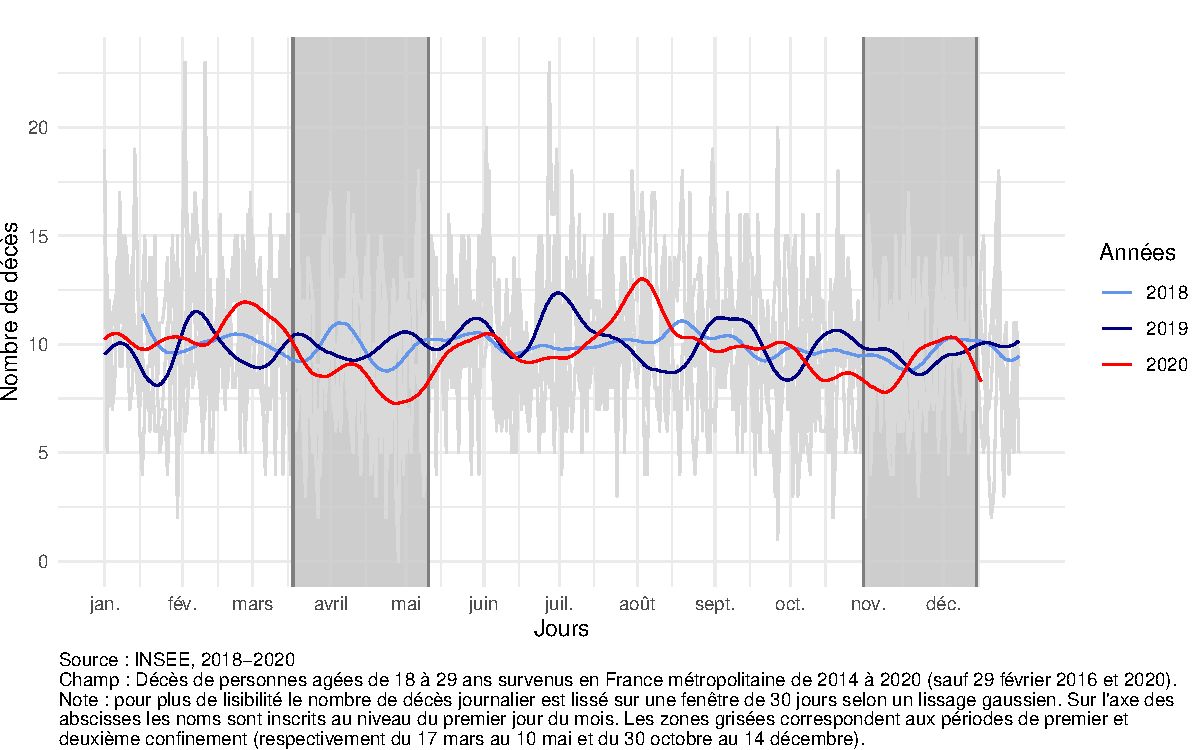
\includegraphics{Aussant_Forcadell_Sessego-courbe_2018_2019}
\end{center}
\caption{Nombre de décès journaliers chez les 18-29 ans en 2018, 2019, et 2020}
\label{fig:courbe_2018_2019}
\end{figure}


\begin{figure}
\begin{center}
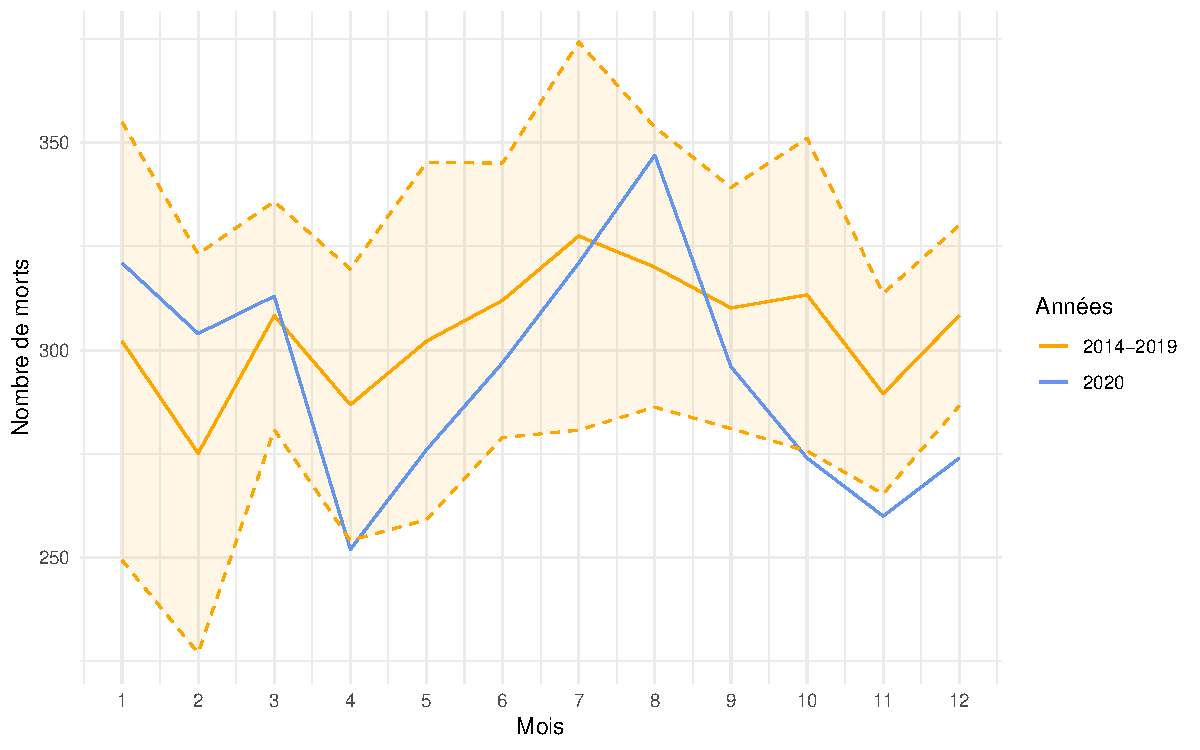
\includegraphics{Aussant_Forcadell_Sessego-courbe_2014_2020}
\end{center}
\caption{Nombre de décès mensuels chez les 18-29 ans entre 2014 et 2020}
\label{fig:courbe_2014_2020}
\end{figure}

% Ne pas oublier de mentionner quelque part que l'on supprime le 29 février de l'analyse

Cela peut s'expliquer par nombreux biais conjoncturels qui peuvent avoir une influence sur la mortalité mais surtout un aléa important car les effectifs des décès parmi les jeunes adultes sont si faibles. C'est ce qui nous a inviter à introduire les années 2014 à 2017 dans la comparaison, bien que nous ne disposons pas du jour exact de décès La Figure 2 présente le nombre de décès par mois en 2020 par rapport à la moyenne des décès par mois de 2014 à 2019 et un intervalle de confiance à 90\%, afin de mettre en évidence une éventuelle tendance sous-jacente au nombre de décès de jeunes adultes par mois. \\

L'on retrouve ici des résultats démontrés dans la littérature : deux pics annuels de mortalité parmi les jeunes, l'un plus faible en hiver (entre janvier et mars sur notre graphique) et l'autre plus important en été (en juillet)  \parencite{breton_levolution_2019}. L'intervalle de confiance demeure important, cependant le nombre de décès au cours des mois d'avril et de novembre-décembre en 2020 (les deux périodes de confinement) ce situent en dehors de celui-ci, ce qui semble confirmer notre hypothèse d'une réduction de la mortalité des jeunes adultes au court des périodes de confinement par rapport aux années précédentes. De plus, la tendance observées pour janvier, février et mars 2020 suivent de manière convaincantes celle des années 2014 à 2019, tendant à conforter l'idée d'une évolution identique de la mortalité entre année avant la survenue du confinement ; nous pouvons donc procéder à une différence de différence. \\

Cependant, en comparant l'évolution du nombre de décès entre mai et septembre pour l'année 2020 par rapport aux années 2014 à 2019, on peut se demander si après la fin des restrictions le confinement ne pourrait pas avoir eu un effet rebond menant à une surmortalité par rapport aux années précédentes. En effet, on observe dans la Figure 2, tout comme dans la Figure 3, une augmentation du nombre de décès de mai à août. On peut en effet supposer que les restrictions imposées lors du confinement, bien qu'elles aient pu avoir un effet protecteur pour les jeunes adultes lors du confinement, ont pu occasionner un effet rebond au cours de la période estivale qui a suivi, où l'intensité des activités à repris de plus belles pour compenser les restrictions des mois précédents. Ainsi, si le confinement a permis de sauver des vies, le même nombre de vie n'a-t-il pas été perdu au court de l'été qui a suivi ? Quel effet du confinement sur le long terme ? \\

Notre postulat d'évolution tendancielle similaire vérifié, il s'agit de procéder la modélisation pour essayer de saisir plus finement cet effet causale, en cherchant en plus de l'effet immédiat du confinement à estimer l'effet du confinement après la fin des restrictions. 

\section*{Modèles et résultats}


%\subsubsection*{Les modèles de régressions choisies}

Nous cherchons à répondre à ces questions à l'aide de différents modèles. Tous cherchent à expliquer le nombre de décès journaliers chez les 18-29 ans en fonction de l'année - 2020 représentant notre groupe « traité », les années précédentes le groupe de contrôle - et de la période considérée - le premier et le deuxième confinement représentant nos périodes de « traitement », les premiers jours de l'année notre période « pré-traitement ». \\

Notre modèle le plus simple s'exprime ainsi de la manière suivante : 

\begin{equation}
\mathrm{Décès}_{it} = \beta_0 + \beta_1 \mathrm{Année}_i + \beta_2 \mathrm{Période}_t + \beta_3 (\mathrm{Année}_i \times \mathrm{Période}_t) + \epsilon_{it}
\end{equation}

où l'indice $i$ renvoie à une année et $t$ à une période. En pratique, le coefficient qui nous intéresse est celui de l'interaction entre l'indicatrice de l'année 2020 et celle de la période de confinement considérée, autrement dit l'estimateur de la différence de différence. Dans le contexte de notre étude, cet estimateur correspond à la différence entre le nombre de décès journaliers attendus en 2020 pendant les périodes de confinement et le nombre réellement observé. \\

Plusieurs ajouts permettent de s'assurer de la robustesse de ce premier modèle et d'améliorer son ajustement. Une première étape consiste à prendre en compte une « effet week-end », selon l'hypothèse que la mortalité des jeunes n'est pas la même - en nombre ou en nature - en début et en fin de semaine.  

\begin{equation}
\begin{aligned}
  \textrm{Décès}_{it} = \beta_0 &+ \beta_1 \textrm{Année}_i + \beta_2 \textrm{Période}_t + \beta_3 (\textrm{Année}_i \times \textrm{Période}_t)\\
   &+ \beta_4 \textrm{Week-end} + \epsilon_{it}
\end{aligned}
\end{equation}

Si la variable indicatrice de week-end peut améliorer l'ajustement de notre modèle, l'ajout d'une interaction de troisième ordre entre année, période, et week-end permet d'affiner notre compréhension de l'effet du confinement sur la mortalité des jeunes. On peut en effet supposer que les décès liés au sorties et comportements à risques sont en temps normal plus fréquents le week-end, et auraient ainsi d'autant plus diminué pendant les week-ends confinés. L'estimateur de différence de différence devient alors plus complexe, puisqu'il se dédouble en une différence dans le nombre de décès attendus et observés en semaine d'une part, pendant le week-end d'autre part, soit les coefficients $\beta_3$ et $\beta_6$ dans le modèle suivant :

\begin{equation}
\begin{aligned}
  \textrm{Décès}_{it} = \beta_0 &+ \beta_1 \textrm{Année}_i + \beta_2 \textrm{Période}_t + \beta_3 (\textrm{Année}_i \times \textrm{Période}_t)\\
   &+ \beta_4 \textrm{Week-end} + \beta_5 (\textrm{Période}_i \times \textrm{Week-end}_t)\\
   &+ \beta_6 (\textrm{Année}_i \times \textrm{Période}_t \times \textrm{Week-end}_t) + \epsilon_{it}
\end{aligned}
\end{equation}

Enfin nos deux derniers modèles reprennent les modèles précédents en leur ajoutant des effets fixes journaliers. Cet ajout vise à contrôler la saisonnalité de la mortalité de manière plus précise que ne peut le faire la variable de période. On considère ainsi les modèles suivant :

\begin{equation}
\begin{aligned}
  \textrm{Décès}_{ijt} = \beta_0 &+ \beta_1 \textrm{Année}_i + \beta_2 \textrm{Période}_t + \beta_3 (\textrm{Année}_i \times \textrm{Période}_t) \\
  &+ \alpha_j + \epsilon_{it}
\end{aligned}
\end{equation}

\begin{equation}
\begin{aligned}
  \textrm{Décès}_{it} = \beta_0 &+ \beta_1 \textrm{Année}_i + \beta_2 \textrm{Période}_t + \beta_3 (\textrm{Année}_i \times \textrm{Période}_t)\\
   &+ \beta_4 \textrm{Week-end} + \beta_5 (\textrm{Période}_i \times \textrm{Week-end}_t)\\
   &+ \beta_6 (\textrm{Année}_i \times \textrm{Période}_t \times \textrm{Week-end}_t) + \alpha_j + \epsilon_{it}
\end{aligned}
\end{equation}

où l'indice $j$ correspond au jour de l'année, et $\alpha_j$ aux effets fixes propres à chaque jour. Par souci de cohérence les 29 février des années bissextiles 2016 et 2020 ne sont pas pris en compte dans les modèles. \\

Dans la mesure où le nombre décès journaliers pour les années 2014 à 2017 ont été imputé à partir du nombre de décès mensuels, nous présentons séparément les régressions effectuées sur les années 2018-2020 puis sur l'ensemble des années 2014 à 2020. Pour les mêmes raisons, les régressions prenant en compte une effet « week-end » n'auraient pas eu de sens pour les années 2014 à 2017 et n'ont dont pas été réalisés. Le modèle 6 correspond ainsi au modèle 4 sans effet weekend, et dans lequel on a également substitué les effets fixes journaliers par des effets fixes mensuels afin de s'adapter au niveau de précision des données disponibles. Par ailleurs, l'imputation du nombre de décès journaliers entraîne une réduction artificielle de la variance des données pour ces années. Les régressions portant sur l'ensemble des années 2014 à 2020 ont ainsi avant tout pour objet de confirmer la robustesse des coefficients observés pour les années 2018 à 2020. Enfin, l'ajout d'effets fixes aux régressions portant sur la période du deuxième confinement n'a pas été techniquement possible, l'information contenue dans les données semblant être insuffisante pour estimer ces modèles.


\subsection*{Une réduction importante de la mortalité des jeunes adultes pendant le premier confinement...}

  L'ensemble des modèles confirment un effet net du premier confinement dans le sens d'une réduction de la mortalité des 18-29 ans par rapport aux années précédentes (Tableau \ref{tab:reg-conf1}). En tenant compte des marges d'erreurs, entre 1 et 4 vies auraient ainsi été « sauvées » chaque jour pendant cette période, soit une réduction de 10 à 40\% des décès en considérant qu'en moyenne 10 jeunes adultes meurent par jour, ce qui est considérable.  Les modèles prenant en compte l'ensemble des années 2014 à 2020  présentent des coefficients très proches de ceux estimés sur les années 2018 à 2020, attestant ainsi de la solidité de ces résultats. Il en va de même après l'ajout d'effet fixe, qui confirme cette robustesse et augmente la capacité explicative des modèles. \\
  
On constate par ailleurs des variations importantes de la mortalité entre les jours de semaine et de week-end. Avant 2020, le nombre de décès est plus élevé le week-end qu'en semaine, avec un peu plus d'un décès de plus en moyenne par jour le weekend. Cet écart est d'autant marqué plus sur la période allant du 17 mars au 10 mai, avec deux décès journaliers de plus contre un en moyenne du premier janvier au 17 mars, probablement car le début du printemps et synonymes de davantage de sorties. L'effet du confinement est donc également différencié en fonction des jours de la semaine et du weekend : l'interaction du troisième ordre entre année, période et week-end montrent que ce sont davantage les décès survenus pendant le week-end (entre 1 et 6 vies « sauvées ») qu'en semaine (entre 0 et 3 vies « sauvées ») qui ont été affectés par la période de confinement de 2020. Ce résultat va dans les sens d'une réduction des activités à risques le week-end chez les jeunes du fait des restrictions sanitaires.   \\


\subsection{... moins spectaculaire si on prend en compte l'effet « déconfinement »}

la Figure \ref{fig:courbe_2014_2020} laisse toutefois penser qu'un pic de mortalité post-confinement serait venu « compenser » le nombre de décès juvéniles évités pendant le confinement. Pour tester cette hypothèse nous reprenons les mêmes modèles en considérant cette fois ensemble le premier confinement et la période d'entre-deux-confinements comme période de traitement (Tableau \ref{tab:reg-per23}). Les tendances mise en évidences par les différents modèles sont les mêmes : la mortalité a baissé par rapport aux années précédentes lorsque l'on considère ensemble la période de premier confinement et la période estivale qui l'a directement suivi, et cette baisse est principalement dû à une réduction du nombre de décès le week-end. Cependant, l'amplitude de ces effets est près de deux fois moindre : le nombre de vies « sauvées »  n'est plus compris qu'entre 0 et 2, tandis que ce nombre était estimé entre 1 et 6 dans les modèle ne prenant en compte que le confinement. Si la mortalité des 18-29 ans a donc bien été réduite par les mesures de confinement, cette baisse semble avoir été en partie « compensée » par une hausse d'autaut plus forte du nombre de décès une fois les restrictions levées, bien que le bilan total reste positif.

\subsection*{Un deuxième confinement moins restrictif ?}

Les premières mesures de confinement ont été assez unanimement suivies par les personnes résidant en France, du fait de leur caractère inédit et de leur application à l'ensemble de la population (à l'exception près des travailleur·euses dit·es « essentiel·les »). Le deuxième confinement n'a pas bénéficié cet effet de nouveauté, et à fait l'objet de nombreuses dérogations notamment au sein des établissements scolaires et dans de nombreux secteurs d'activité. Ce confinement moins restrictif a-t-il eu le même effet bénéfique que le premier sur la mortalité des jeunes ? Les résultats des modèles apparaissent peu robustes et ne permettent pas de répondre à cette interrogation de manière certaine (Tableau \ref{tab:reg-conf2}). Seul la régression appliquée aux années 2014 à 2020 fait apparaître une réduction significative du nombre de décès sur la période du deuxième confinement, mais la fiabilité de ces résultats n'est pas assurée du fait de l'imprécision des données mobilisées. L'effet du second confinement serait de toute façon plus limité, avec une réduction des décès journaliers estimés entre  0 et 2 sur la seule période de confinement, contre 1 à 4 pour le premier confinement. Ces résultats restent incertains laissent penser que l'effet du deuxième confinement sur la mortalité des 18-29 ans a été moins important que celui du premier, voire presque inexistants. 


\subsection*{Moins de décès chez les jeunes hommes pendant les week-end du confinement}

La comparaison entre hommes et femmes est particulièrement éclairante et tout à fait en accord avec la littérature citée en introduction. On voit dans le tableau \ref{tab:reg-sexe} que dans tous les cas considérés, l'effet protecteur du confinement est plus important chez les hommes. Sans contrôler par l'effet weekend (modèle 4), on voit une baisse de la mortalité journalière moyenne deux fois plus importante chez les hommes que chez les femmes (en moyenne presque deux vie sauvées par jour pour les hommes contre une pour les femmes). Cela dit, les intervalles de confiances invitent à la prudence, les deux intervalles se recoupant assez largement. \\

En revanche, l'effet weekend différentié selon le sexe ne trompe pas. On n'observe pas de baisse significative de la mortalité journalière les weekends du premier confinement chez les femmes. Il semblerait donc que pour les femmes les vies sauvées ne soient pas plus importantes le weekend que la semaine, avec un coefficient significatif de moins de près de moins un décès par jour pour les femmes. Au contraire, pour les hommes, seuls l'effet weekend apparaît significatif une fois introduit : on observe ainsi une baisse des décès journalier le weekend entre 1,9 et 7,1, un intervalle de confiance à 95 \% strictement distinct de celui des femmes. Ainsi le confinement n'aurait chez les hommes pas diminué le nombre de décès la semaine, mais uniquement le weekend. L'hypothèse d'une baisse de la mortalité dûes avant tout aux pratiques de pratique risqués proprement masculine qui sont plus courantes les weekends (typiquement, la conduite en état d'ébriété) trouve ici un argument statistique convaincant.  \\

Le faible effectif de décès féminins invite à la plus grande prudence pour l'interprétation de nos résultats. En effet, nos données ne permettent pas d’affirmer que l’effet du confinement a été réellement plus fort sur les hommes, si ce n’est lors des weekends. Le taux de décès journalier féminin étant à l’origine beaucoup plus faible, il est normal d’observer une variation en valeur absolue plus faible chez elles, même si l’effet propre éventuel est potentiellement similaire à celui des hommes lors de la semaine. On souffre ici de l’imprécision des estimateurs dû aux faibles effectifs.



\begin{landscape}
\begin{table}[H]

\caption{\label{tab:reg-conf1}Effet du premier confinement sur le nombre de décès journaliers des 18-29 ans}
\centering
\resizebox{\linewidth}{!}{
\fontsize{10}{12}\selectfont
\begin{threeparttable}
\begin{tabular}[t]{lccccccc}
\toprule
\multicolumn{1}{c}{\textbf{}} & \multicolumn{5}{c}{\textbf{2018-2020}} & \multicolumn{2}{c}{\textbf{2014-2020}} \\
\cmidrule(l{3pt}r{3pt}){2-6} \cmidrule(l{3pt}r{3pt}){7-8}
  & (1) & (2) & (3) & (4) & (5) & (1) & (6)\\
\midrule
Intercept & 10.23*** & 9.85*** & 9.9*** &  &  & 10.1*** & \\
 & (9.54 ; 10.92) & (9.14 ; 10.56) & (9.16 ; 10.65) &  &  & (9.68 ; 10.51) & \\
2019 & -0.34 & -0.34 & -0.32 & -0.34 & -0.32 & -0.25 & -0.25\\
 & (-1.17 ; 0.5) & (-1.16 ; 0.48) & (-1.14 ; 0.49) & (-1.15 ; 0.47) & (-1.12 ; 0.47) & (-0.8 ; 0.3) & (-0.8 ; 0.3)\\
2020 & 0.58 & 0.57 & 0.75 & 0.61 & 0.61 & 0.72** & 0.72**\\
 & (-0.46 ; 1.62) & (-0.45 ; 1.6) & (-0.42 ; 1.91) & (-0.41 ; 1.62) & (-0.62 ; 1.84) & (0.06 ; 1.38) & (0.06 ; 1.38)\\
17 mars - 10 mai & -0.14 & -0.15 & -0.73 & 4.28 & 1.44 & -0.04 & 0.19\\
 & (-0.99 ; 0.7) & (-0.99 ; 0.68) & (-1.7 ; 0.24) & (-3.77 ; 12.32) & (-6.73 ; 9.6) & (-0.36 ; 0.29) & (-0.43 ; 0.81)\\
\textbf{2020 × 17 mars - 10 mai} & \textbf{-2.56***} & \textbf{-2.57***} & \textbf{-1.66*} & \textbf{-2.54***} & \textbf{-1.46} & \textbf{-2.67***} & \textbf{-2.67***}\\
\textbf{} & \textbf{(-4.03 ; -1.1)} & \textbf{(-4.01 ; -1.12)} & \textbf{(-3.35 ; 0.02)} & \textbf{(-3.97 ; -1.11)} & \textbf{(-3.26 ; 0.33)} & \textbf{(-3.53 ; -1.81)} & \textbf{(-3.52 ; -1.81)}\\
Week-end &  & 1.39*** & 1.16* &  & 1 &  & \\
 &  & (0.64 ; 2.14) & (-0.04 ; 2.37) &  & (-0.56 ; 2.57) &  & \\
17 mars - 10 mai × week-end &  &  & 2.04** &  & 1.83 &  & \\
 &  &  & (0.2 ; 3.88) &  & (-0.59 ; 4.26) &  & \\
2020 × 1 jan - 16 mars × week-end &  &  & -0.57 &  & -0.01 &  & \\
 &  &  & (-2.65 ; 1.5) &  & (-2.59 ; 2.57) &  & \\
\textbf{2020 × 17 mars - 10 mai × week-end} & \textbf{} & \textbf{} & \textbf{-3.71***} & \textbf{} & \textbf{-3.95**} & \textbf{} & \textbf{}\\
\textbf{} & \textbf{} & \textbf{} & \textbf{(-6.11 ; -1.32)} & \textbf{} & \textbf{(-7.03 ; -0.87)} & \textbf{} & \textbf{}\\
2015 &  &  &  &  &  & -0.43 & -0.43\\
 &  &  &  &  &  & (-0.98 ; 0.12) & (-0.98 ; 0.12)\\
2016 &  &  &  &  &  & -0.52* & -0.52*\\
 &  &  &  &  &  & (-1.07 ; 0.04) & (-1.07 ; 0.04)\\
2017 &  &  &  &  &  & -0.74*** & -0.74***\\
 &  &  &  &  &  & (-1.3 ; -0.19) & (-1.3 ; -0.19)\\
2018 &  &  &  &  &  & 0.09 & 0.09\\
 &  &  &  &  &  & (-0.47 ; 0.64) & (-0.47 ; 0.64)\\
Observations & 390 & 390 & 390 & 390 & 390 & 910 & 910\\
R2 & 0.052 & 0.084 & 0.111 & 0.413 & 0.440 & 0.060 & 0.065\\
R2 ajusté & 0.043 & 0.072 & 0.092 & 0.104 & 0.132 & 0.052 & 0.052\\
\bottomrule
\end{tabular}
\begin{tablenotes}
\item Source : INSEE, 2014 à 2020.
\item Champ : décès journaliers de personnes agées de 18 à 29 ans survenus en France métropolitaine entre 2014 et 2020, sur la période du 1er janvier au 10 mai.
\item Seuils de significativité : p < 0,1 *; p < 0,05 **, p < 0,01 ***.
\end{tablenotes}
\end{threeparttable}}
\end{table}\end{landscape}

\begin{landscape}
\begin{table}[H]

\caption{\label{tab:reg-per23}Effet du premier confinement et de la période d'entre-deux-confinements sur le nombre de décès journaliers des 18-29 ans}
\centering
\resizebox{\linewidth}{!}{
\fontsize{10}{12}\selectfont
\begin{threeparttable}
\begin{tabular}[t]{lccccccc}
\toprule
\multicolumn{1}{c}{\textbf{}} & \multicolumn{5}{c}{\textbf{2018-2020}} & \multicolumn{2}{c}{\textbf{2014-2020}} \\
\cmidrule(l{3pt}r{3pt}){2-6} \cmidrule(l{3pt}r{3pt}){7-8}
  & (1) & (2) & (3) & (4) & (5) & (1) & (6)\\
\midrule
Intercept & 10.08*** & 9.69*** & 9.76*** &  &  & 10.04*** & \\
 & (9.47 ; 10.69) & (9.07 ; 10.3) & (9.08 ; 10.44) &  &  & (9.72 ; 10.36) & \\
2019 & -0.04 & -0.04 & -0.03 & -0.04 & -0.03 & -0.27 & -0.27\\
 & (-0.58 ; 0.51) & (-0.57 ; 0.5) & (-0.57 ; 0.5) & (-0.57 ; 0.49) & (-0.56 ; 0.5) & (-0.64 ; 0.09) & (-0.63 ; 0.09)\\
2020 & 0.74 & 0.73 & 0.89 & 0.75 & 0.75 & 0.77** & 0.77**\\
 & (-0.25 ; 1.72) & (-0.24 ; 1.69) & (-0.24 ; 2.01) & (-0.21 ; 1.72) & (-0.46 ; 1.97) & (0.17 ; 1.38) & (0.17 ; 1.37)\\
17 mars - 29 oct & 0.01 & -0.02 & -0.27 & 3.12 & 2.38 & 0.37*** & 0.04\\
 & (-0.62 ; 0.64) & (-0.64 ; 0.6) & (-0.99 ; 0.46) & (-4.95 ; 11.18) & (-5.72 ; 10.49) & (0.13 ; 0.61) & (-0.57 ; 0.65)\\
\textbf{2020 × 17 mars - 29 oct} & \textbf{-1.25**} & \textbf{-1.23**} & \textbf{-0.98} & \textbf{-1.26**} & \textbf{-0.74} & \textbf{-1.61***} & \textbf{-1.61***}\\
\textbf{} & \textbf{(-2.34 ; -0.15)} & \textbf{(-2.3 ; -0.15)} & \textbf{(-2.24 ; 0.28)} & \textbf{(-2.33 ; -0.19)} & \textbf{(-2.1 ; 0.63)} & \textbf{(-2.26 ; -0.97)} & \textbf{(-2.25 ; -0.97)}\\
Week-end &  & 1.42*** & 1.16* & 1.15*** & 0.99 &  & \\
 &  & (0.94 ; 1.91) & (-0.04 ; 2.36) & (0.54 ; 1.76) & (-0.59 ; 2.58) &  & \\
17 mars - 29 oct × week-end &  &  & 0.88 &  & 0.89 &  & \\
 &  &  & (-0.5 ; 2.26) &  & (-0.93 ; 2.72) &  & \\
2020 × 1 jan - 16 mars × week-end &  &  & -0.57 &  & 0 &  & \\
 &  &  & (-2.64 ; 1.5) &  & (-2.62 ; 2.61) &  & \\
\textbf{2020 × 17 mars - 29 oct × week-end} & \textbf{} & \textbf{} & \textbf{-1.43**} & \textbf{} & \textbf{-1.83**} & \textbf{} & \textbf{}\\
\textbf{} & \textbf{} & \textbf{} & \textbf{(-2.61 ; -0.24)} & \textbf{} & \textbf{(-3.34 ; -0.32)} & \textbf{} & \textbf{}\\
2015 &  &  &  &  &  & -0.1 & -0.1\\
 &  &  &  &  &  & (-0.46 ; 0.27) & (-0.46 ; 0.27)\\
2016 &  &  &  &  &  & -0.3 & -0.3\\
 &  &  &  &  &  & (-0.67 ; 0.06) & (-0.66 ; 0.06)\\
2017 &  &  &  &  &  & -0.61*** & -0.61***\\
 &  &  &  &  &  & (-0.98 ; -0.25) & (-0.97 ; -0.25)\\
2018 &  &  &  &  &  & -0.24 & -0.24\\
 &  &  &  &  &  & (-0.6 ; 0.13) & (-0.6 ; 0.13)\\
Observations & 906 & 906 & 906 & 906 & 906 & 2114 & 2114\\
R2 & 0.009 & 0.044 & 0.052 & 0.377 & 0.383 & 0.019 & 0.041\\
R2 ajusté & 0.004 & 0.039 & 0.043 & 0.057 & 0.061 & 0.015 & 0.033\\
\bottomrule
\end{tabular}
\begin{tablenotes}
\item Source : INSEE, 2014 à 2020.
\item Champ : décès journaliers de personnes agées de 18 à 29 ans survenus en France métropolitaine entre 2014 et 2020, sur la période du 1er janvier au 29 octobre.
\item Seuils de significativité : p < 0,1 *; p < 0,05 **, p < 0,01 ***.
\end{tablenotes}
\end{threeparttable}}
\end{table}\end{landscape}

% \begin{landscape}
% \end{landscape}


\begin{landscape}
\begin{table}[H]

\caption{\label{tab:reg-conf2}Effet du deuxième confinement sur le nombre de décès journaliers des 18-29 ans}
\centering
\fontsize{10}{12}\selectfont
\begin{threeparttable}
\begin{tabular}[t]{lcccc}
\toprule
\multicolumn{1}{c}{\textbf{}} & \multicolumn{3}{c}{\textbf{2018-2020}} & \multicolumn{1}{c}{\textbf{2014-2020}} \\
\cmidrule(l{3pt}r{3pt}){2-4} \cmidrule(l{3pt}r{3pt}){5-5}
  & (1) & (2) & (3) & (1)\\
\midrule
Intercept & 10.32*** & 10.23*** & 10*** & 10.02***\\
 & (9.64 ; 11) & (9.52 ; 10.94) & (9.25 ; 10.75) & (9.61 ; 10.44)\\
2019 & -0.52 & -0.53 & -0.52 & -0.45\\
 & (-1.36 ; 0.32) & (-1.37 ; 0.31) & (-1.36 ; 0.31) & (-1 ; 0.11)\\
2020 & 0.49 & 0.49 & 0.65 & 0.79**\\
 & (-0.52 ; 1.51) & (-0.53 ; 1.5) & (-0.51 ; 1.81) & (0.14 ; 1.44)\\
30 oct - 14 déc & -0.65 & -0.65 & -0.09 & -0.06\\
 & (-1.51 ; 0.22) & (-1.51 ; 0.22) & (-1.1 ; 0.92) & (-0.39 ; 0.28)\\
\textbf{2020 × 30 oct - 14 déc} & \textbf{-0.8} & \textbf{-0.81} & \textbf{-1.09} & \textbf{-1.39***}\\
\textbf{} & \textbf{(-2.29 ; 0.7)} & \textbf{(-2.3 ; 0.69)} & \textbf{(-2.86 ; 0.68)} & \textbf{(-2.26 ; -0.51)}\\
Week-end &  & 0.34 & 1.17* & \\
 &  & (-0.43 ; 1.1) & (-0.02 ; 2.36) & \\
30 oct - 14 déc × week-end &  &  & -2.05** & \\
 &  &  & (-3.99 ; -0.11) & \\
2020 × 1 jan - 16 mars × week-end &  &  & -0.58 & \\
 &  &  & (-2.63 ; 1.48) & \\
\textbf{2020 × 30 oct - 14 déc × week-end} & \textbf{} & \textbf{} & \textbf{0.56} & \textbf{}\\
\textbf{} & \textbf{} & \textbf{} & \textbf{(-2.03 ; 3.14)} & \textbf{}\\
2015 &  &  &  & -0.13\\
 &  &  &  & (-0.69 ; 0.42)\\
2016 &  &  &  & -0.19\\
 &  &  &  & (-0.75 ; 0.36)\\
2017 &  &  &  & -0.71**\\
 &  &  &  & (-1.27 ; -0.16)\\
2018 &  &  &  & 0.07\\
 &  &  &  & (-0.48 ; 0.63)\\
Observations & 363 & 363 & 363 & 847\\
R2 & 0.029 & 0.031 & 0.044 & 0.033\\
R2 ajusté & 0.018 & 0.017 & 0.022 & 0.024\\
\bottomrule
\end{tabular}
\begin{tablenotes}
\item Source : INSEE, 2014 à 2020.
\item Champ : décès journaliers de personnes agées de 18 à 29 ans survenus en France métropolitaine entre 2014 et 2020, sur la période du 1er janvier au 16 mars et du 30 octobre au 14 décembre.
\item Seuils de significativité : p < 0,1 *; p < 0,05 **, p < 0,01 ***.
\end{tablenotes}
\end{threeparttable}
\end{table}\end{landscape}


\begin{landscape}
\begin{table}[H]

\caption{\label{tab:reg-sexe}Effet différencié du premier confinement sur le nombre de décès journaliers des 18-29 ans chez les femmes et chez les hommes}
\centering
\resizebox{\linewidth}{!}{
\fontsize{10}{12}\selectfont
\begin{threeparttable}
\begin{tabular}[t]{lcccccc}
\toprule
\multicolumn{1}{c}{\textbf{}} & \multicolumn{3}{c}{\textbf{Femmes}} & \multicolumn{3}{c}{\textbf{Hommes}} \\
\cmidrule(l{3pt}r{3pt}){2-4} \cmidrule(l{3pt}r{3pt}){5-7}
\multicolumn{1}{c}{} & \multicolumn{2}{c}{2018-2019} & \multicolumn{1}{c}{2014-2019} & \multicolumn{2}{c}{2018-2019} & \multicolumn{1}{c}{2014-2019} \\
\cmidrule(l{3pt}r{3pt}){2-3} \cmidrule(l{3pt}r{3pt}){4-4} \cmidrule(l{3pt}r{3pt}){5-6} \cmidrule(l{3pt}r{3pt}){7-7}
  & (4) & (5) & (4) & (4) & (5) & (4)\\
\midrule
2019 & -0.12 & -0.12 & 0.06 & -0.22 & -0.2 & -0.31\\
 & (-0.54 ; 0.29) & (-0.54 ; 0.29) & (-0.22 ; 0.34) & (-0.91 ; 0.48) & (-0.87 ; 0.47) & (-0.78 ; 0.15)\\
2020 & 0.2 & 0.11 & 0.43** & 0.41 & 0.51 & 0.3\\
 & (-0.31 ; 0.72) & (-0.54 ; 0.75) & (0.1 ; 0.77) & (-0.46 ; 1.27) & (-0.53 ; 1.55) & (-0.25 ; 0.86)\\
17 mars - 10 mai & 2.26 & 2.34 & 1.22 & 2.01 & -0.9 & 0.89\\
 & (-1.84 ; 6.37) & (-1.92 ; 6.59) & (-0.68 ; 3.12) & (-4.88 ; 8.91) & (-7.79 ; 6) & (-2.25 ; 4.03)\\
\textbf{2020 × 17 mars - 10 mai} & \textbf{-0.8**} & \textbf{-0.86*} & \textbf{-0.95***} & \textbf{-1.74***} & \textbf{-0.6} & \textbf{-1.7***}\\
\textbf{} & \textbf{(-1.53 ; -0.07)} & \textbf{(-1.79 ; 0.08)} & \textbf{(-1.38 ; -0.51)} & \textbf{(-2.96 ; -0.51)} & \textbf{(-2.12 ; 0.91)} & \textbf{(-2.42 ; -0.98)}\\
Week-end &  & -0.14 &  &  & 1.14* & \\
 &  & (-0.96 ; 0.67) &  &  & (-0.18 ; 2.46) & \\
17 mars - 10 mai × week-end &  & -0.03 &  &  & 1.86* & \\
 &  & (-1.29 ; 1.23) &  &  & (-0.18 ; 3.91) & \\
2020 × 1 jan - 16 mars × week-end &  & 0.34 &  &  & -0.35 & \\
 &  & (-1 ; 1.69) &  &  & (-2.53 ; 1.83) & \\
\textbf{2020 × 17 mars - 10 mai × week-end} & \textbf{} & \textbf{0.55} & \textbf{} & \textbf{} & \textbf{-4.51***} & \textbf{}\\
\textbf{} & \textbf{} & \textbf{(-1.05 ; 2.16)} & \textbf{} & \textbf{} & \textbf{(-7.11 ; -1.91)} & \textbf{}\\
2015 &  &  & -0.03 &  &  & -0.4*\\
 &  &  & (-0.31 ; 0.25) &  &  & (-0.86 ; 0.06)\\
2016 &  &  & -0.12 &  &  & -0.37\\
 &  &  & (-0.41 ; 0.16) &  &  & (-0.83 ; 0.1)\\
2017 &  &  & -0.18 &  &  & -0.57**\\
 &  &  & (-0.46 ; 0.1) &  &  & (-1.03 ; -0.1)\\
2018 &  &  & 0.18 &  &  & -0.1\\
 &  &  & (-0.1 ; 0.46) &  &  & (-0.56 ; 0.37)\\
Observations & 390 & 390 & 910 & 390 & 390 & 910\\
R2 & 0.412 & 0.414 & 0.209 & 0.379 & 0.424 & 0.180\\
R2 ajusté & 0.103 & 0.091 & 0.068 & 0.052 & 0.108 & 0.033\\
\bottomrule
\end{tabular}
\begin{tablenotes}
\item Source : INSEE, 2014 à 2020.
\item Champ : décès journaliers de personnes agées de 18 à 29 ans survenus en France métropolitaine entre 2014 et 2020, sur la période du 1er janvier au 10 mai.
\item Seuils de significativité : p < 0,1 *; p < 0,05 **, p < 0,01 ***.
\end{tablenotes}
\end{threeparttable}}
\end{table}
\end{landscape}

\section*{Conclusion - une baisse de la mortalité des jeunes adultes, des mécanismes à préciser}

Les modèles développés dans cet étude tendent à confirmer un effet causal substantiel du premier confinement sur la mortalité journalière des 18–29 ans, allant d'un peu plus de deux vies sauvées en moyenne par jour durant la période de confinement, à un peu plus d'une, si on prend en considération le rebond de mortalité durant l'été suivant le déconfinement ; un effet important, représentant près de 10\% des décès des jeunes adultes durant cette période.Il semblerait donc que les restrictions de déplacement aient eu un effet protecteur bien plus important qu'un éventuel risqus accru de suicide liés à l'isolation (bien que l'accroissement de ce risque reste fortement débattu, le confinement ayant pu avoir un effet protecteur envers le suicide \parencite{letourneur_suicide_2022,olie_hospitalizations_2021}) - le suicide demeure en effet une des causes de décès les plus importantes parmi cette tranche d'âge (INSERM, 2020).  \\

Cet effet protecteur du confinement semble avoir en premier lieu permis d'éviter des décès de jeunes hommes durant les weekends, et dans une moindre mesure ceux des jeunes femmes. Cela tend à confirmer notre hypothèse que cette baisse de mortalité soit avant tout due à une baisse de la mortalité violente (par accidents, notamment dûes aux sortie le weekend). Cependant, en attendant des données par cause de décès produites par l'INSERM (un travail de codification de longue haleine qui prendra encore au moins une année \parencite{gastineau_lepidemie_2022}), il est difficile d'affirmer avec certitude les mécanismes expliquant cette diminution des décès chez les jeunes adultes. \\

Enfin, l'effet du second confinement semble avoir été bien moins important que celui du premier, voir inexistant. Cependant, la faiblesse des effectifs considérés ne nous permet pas d'affirmer avec certitude l'existence ou l'absence d'un effet. De manière générale, l'hypothèse fondamentale pour le modèle de différence de différence reste difficile à démontrer avec une grande précision, du fait la faiblesse de la mortalité des jeunes et donc de la forte volatilité des effectifs, et de l'absence des données journalières les années 2017 à 2014. Elle reste cependant crédible, mais invite à interpréter les résultats davantage en terme d'ordre de grandeur plutôt que dans leurs détails. Par ailleurs, il aurait pu être intéressant de faire varier les périodes testés, notamment en s'interrogeant sur un respect plus ou moins effectif du confinement en début ou fin de période. Mais nous sommes à nouveau est limité par les effectifs, qui offre peu de latitude pour découper de manière plus fine la population.

% En toute rigueur, on ne peut en l’état affirmer de manière absolument ferme que les variations mesurées ne sont pas dû à un aléa inobservé propre à l’année 2020 non relatif au confinement. Tout dispositif d’identification causal, qu’il soit expérimental ou pseudo expérimental comme ici contient une part d’incertitude quant à l’existence de facteurs de confusion non pris en compte. Cela étant, le fait qu’on observe une baisse de la mortalité uniquement lors du confinement le plus stricte (le premier) et particulièrement le weekend chez les hommes, cela de manière cohérente avec certaines observations formulées dans la littérature consacrée à la mortalité des jeunes, confère une bonne crédibilité au schéma d’analyse présenté, au-delà de l’argumentation purement statistique. Dans cette perspective, disposer des causes de décès aurait pu permettre d’affiner nos conclusions, notamment concernant la place de la mortalité routière, qu’on a supposé être l’une des premières causes concernées par l’effet du confinement. Par ailleurs il aurait pu être intéressant de faire varier les périodes testés, notamment en s'interrogeant sur un respect plus ou moins effectif du confinement en début ou fin de période. A nouveau, on est limité par les effectifs qui offre peu de latitude pour découper de manière plus fine la population.




\section*{Sources} 
\label{source}

\begin{itemize}
\item INSEE, 2022, \url{https://www.insee.fr/fr/outil-interactif/5014911/pyramide.htm#!y=2015&a=18,30&v=2&c=0}

\item INSEE, 2020, \url{https://www.insee.fr/fr/statistiques/5431034?sommaire=5419788&q=d\%C3\%A9c\%C3\%A8s+2020}
\item INSEE, 2019, \url{https://www.insee.fr/fr/statistiques/4801913?sommaire=4768339&q=d\%C3\%A9c\%C3\%A8s+2019}
\item INSEE, 2018, \url{https://www.insee.fr/fr/statistiques/4216603?sommaire=4215184}
\item INSEE, 2017, \url{https://www.insee.fr/fr/statistiques/3606190?sommaire=3596198}
\item INSEE, 2016, \url{https://www.insee.fr/fr/statistiques/3053349?sommaire=3051496}
\item INSEE, 2015, \url{https://www.insee.fr/fr/statistiques/2406453?sommaire=2406457}
\item INSEE, 2014, \url{https://www.insee.fr/fr/statistiques/2114975?sommaire=2114983}

\item INSERM, 2020 \url{http://cepidc-data.inserm.fr/inserm/html/index2.htm}
\end{itemize}

\printbibliography



\end{document}
